%
% File: chap06.tex
%
\let\textcircled=\pgftextcircled
\chapter{Functional models}
\label{chap:fm}

\newacronym{fbed}{FBED}{Functional Basis for Engineering Design}
\newacronym{ffip}{FFIP}{Funtion Failure Identification and Propagation}
\newacronym{ffdm}{FFDM}{Function Failure Design Method}
\newacronym{uffsr}{UFFSR}{Uncoupled Flow Failure State Reasoning}

\initial{A} different way of representing an engineering system is to embed it as a functional model. A functional model is a graphical representation of a system, that ties a component to a function, or a set of functions, fulfilled within the system. Function are interconnected by flows. One of the main advantage of functional modeling is its applicability in the early stages of design, when no components have been selected and the design is just a concept. Until recently, two main methods existed to create a functional method, NIST and ?. Each had their own volatile taxonomy, which limited the widespread use of this technique to other ends than system description. Stone and Wood proposed the \gls{fbed}~\cite{stone}, which reconciled sets of function and flows notably with relation to mechanical engineering design nomenclature. This common taxonomy allowed for automatic analysis methods and database maintenance, which paved the way to various risk and reliability methods based on functional models, such as \gls{ffdm}~\cite{stone2005}, \gls{ffip}~\cite{kurtoglu2007} or \gls{uffsr}~\cite{vanbossuyt2014},~\cite{ohalloran2015}.


\section{Functional model}

A FBED description of a system uses the reconciled function set and flow set to name the various functions and flows necessary within a system. Tables~\ref{tab:fbed_func} and~\ref{tab:fbed_flow} give a few example of such functions and flows. FBED is organized using three classes, primary, secondary and tertiary, each increasing the degree of specification. THose three classes cover every potential function seen in a mechanical design. It is to be noted that it still allow for some level of interpretation as to how to categorize a function or flow.

A FBED model can be compared to a RBD. They both can take various degrees of details, high-level to low-level model description. One of the advantages that FBED exhibits as opposed to RBD is that it considers explicitely the flows linking the different functions. Moreover, it does not depend on the component selection, which allow the design team to explore a larger space of possible systems. Figure~\ref{fig:fbed} show an example of a functional model applied to the present case study. One can note that the level of details can be modified. Moreoever, to simplify the drawing, the redundancies displayed by the system are not explicited as separate functions and flows. They are instead encoded within the probabilities associated with each function or flow failure propagation.

\renewcommand{\arraystretch}{1.2}
\begin{table}[t] \small
\centering
\caption{Excerpt from the functional basis reconciled function set}
\label{tab:fbed_func}
\begin{tabular}{|c|c|c|}
\hline
Class (primary)          & Secondary                 & Tertiary  \\ \hline
\multirow{4}{*}{Branch}  & \multirow{3}{*}{Separate} & Divide    \\ \cline{3-3} 
                         &                           & Extract   \\ \cline{3-3} 
                         &                           & Remove    \\ \cline{2-3} 
                         & Distribute                &           \\ \hline
\multirow{7}{*}{Channel} & Import                    &           \\ \cline{2-3} 
                         & Export                    &           \\ \cline{2-3} 
                         & \multirow{2}{*}{Transfer} & Transport \\ \cline{3-3} 
                         &                           & Transmit  \\ \cline{2-3} 
                         & \multirow{3}{*}{Guide}    & Translate \\ \cline{3-3} 
                         &                           & Rotate    \\ \cline{3-3} 
                         &                           & Allow DOF \\ \hline
\multicolumn{3}{|c|}{...}                                        \\ \hline
Support & Position &           \\ \hline
\end{tabular}
\end{table}

\begin{table}[t] \small
\centering
\caption{Excerpt from the functional basis reconciled flow set}
\label{tab:fbed_flow}
\begin{tabular}{|c|c|c|}
\hline
Class (primary)              & Secondary                    & Tertiary                         \\ \hline
\multirow{6}{*}{Material}    & Human                        &                                  \\ \cline{2-3} 
                             & Gas                          &                                  \\ \cline{2-3} 
                             & Liquid                       &                                  \\ \cline{2-3} 
                             & \multirow{3}{*}{Solid}       & Object                           \\ \cline{3-3} 
                             &                              & \multicolumn{1}{l|}{Particulate} \\ \cline{3-3} 
                             &                              & \multicolumn{1}{l|}{Composite}   \\ \hline
\multicolumn{3}{|c|}{...}                                                                      \\ \hline
Energy & Thermal &             \\ \hline
\end{tabular}
\end{table}

\begin{figure}[t]
\centering
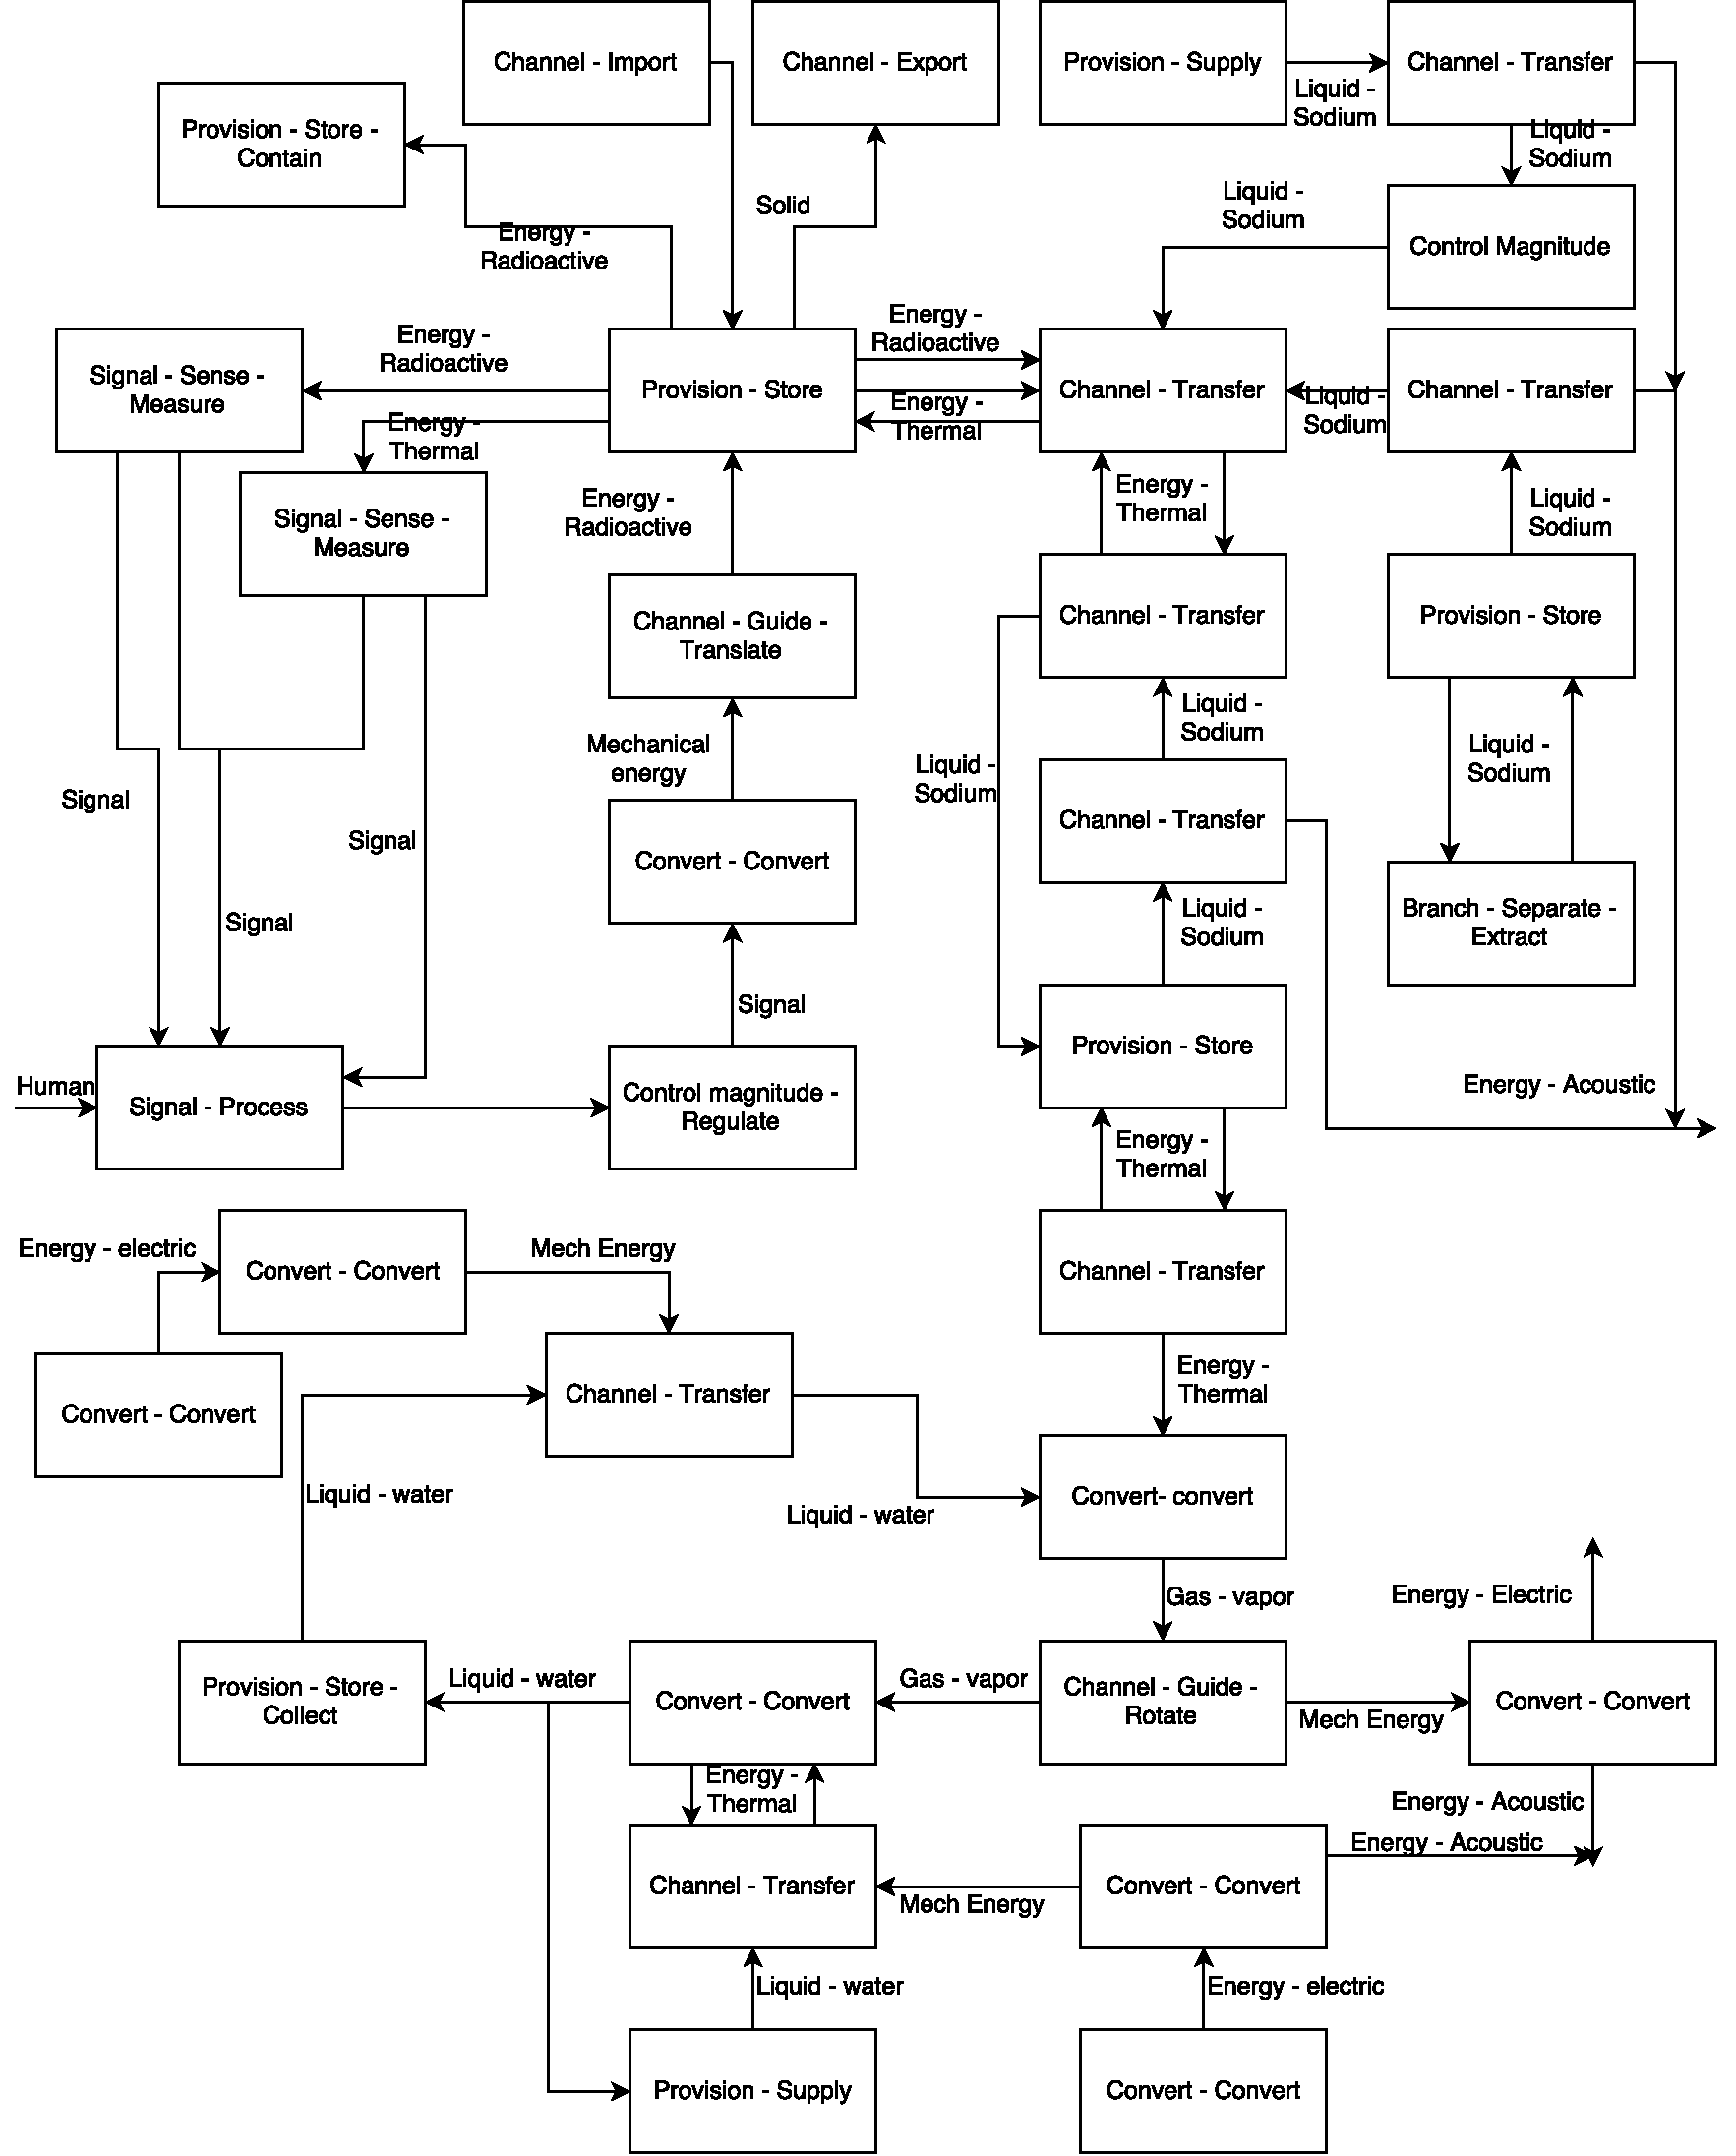
\includegraphics[scale=.6]{fig/Functional_model}
\caption{High-level simplified FBED representation of ASTRID reactor.}
\label{fig:fbed}
\end{figure}

\section{Function Failure Design Method}

FFDM is a method whose main goal is to look at historical component failure data within a system, and estimate the different failure mode observed. Those failure modes are then linked to the functions in the design. Effectively, FFDM is similar to FMEA, but allow for a more generalized approach by taking on functions. The failure modes identified can then be mitigated by modifying the functions used in the system. It has been shown that given the right database available, FFDM gave more information on the potential risk and possible actions to mitigate them in a system than FMEA. Moreover, being based on functions-failure-modes database, this method is less likely to depend uniquely on expert opinion.

To illustrate this method, let us assume that a repository of failure modes for a given system is available. An engineering team wants to improve upon the original design, or create a new design entirely. The first step is to translate the system to a functional black-box model. Then, for each function, the failure history is analyzed, and a suceptibility score is used to link a function to all potential failure mode. Given that information, a mitigation analysis is conducted, allowing to choose the most adequate components addressing the identified function failure modes.

The fact that this method is based upon functional model allow for its use in conceptual design. One of its limitation is the existence of a complete database, and the fact that a function can fail following different failure modes depending on operating stresses and component physical attributes.

Table~\ref{tab:ffdm_dat} shows several failure modes occurences for a subset of the case study system functions.

\begin{table}[t] \small
\centering
\caption{FFDM database}
\label{tab:ffdm_dat}
\begin{tabular}{|c|c|c|c|c|l|c|}
\hline
Function/Failure            & \begin{tabular}[c]{@{}c@{}}Corrosion\\ Fatigue\end{tabular} & \begin{tabular}[c]{@{}c@{}}Direct\\ Chemical \\ Attack\end{tabular} & \begin{tabular}[c]{@{}c@{}}High\\ Cycle\\ Fatigue\end{tabular} & \begin{tabular}[c]{@{}c@{}}Thermal\\ Shock\end{tabular} & \multirow{8}{*}{...} & Yielding \\ \cline{1-5} \cline{7-7} 
Channel - Transfer          & 0                                                           & 0                                                                   & 0                                                              & 0                                                       &                      & 0        \\ \cline{1-5} \cline{7-7} 
Provision - Store - Contain & 0                                                           & 0                                                                   & 0                                                              & 0                                                       &                      & 0        \\ \cline{1-5} \cline{7-7} 
Signal - Sense - Measure    & 0                                                           & 0                                                                   & 0                                                              & 0                                                       &                      & 0        \\ \cline{1-5} \cline{7-7} 
Convert - Convert           & 0                                                           & 0                                                                   & 0                                                              & 0                                                       &                      & 0        \\ \cline{1-5} \cline{7-7} 
Branch - Separate - Extract & 0                                                           & 0                                                                   & 0                                                              & 0                                                       &                      & 0        \\ \cline{1-5} \cline{7-7} 
Channel - Guide - Translate & 0                                                           & 0                                                                   & 0                                                              & 0                                                       &                      & 0        \\ \cline{1-5} \cline{7-7}
\multicolumn{7}{|c|}{...}                                                                                                                                                                                                                                                                                                    \\ \hline
\end{tabular}
\end{table}

